\documentclass[tikz]{standalone}
\usepackage{tikz}
\usepackage{pgfplots}
\usepackage{pgf-spectra}
\usetikzlibrary{arrows}
\usetikzlibrary{decorations.markings}

\tikzset{>=latex}

\tikzset{linha/.style={line width=7pt,MaterialGrey300}}

\def \plotwidth {510.0pt}
\def \tth{3.16227766017}

\definecolor{color1}{RGB}{202,0,32}
\definecolor{color2}{RGB}{244,165,130}
\definecolor{color3}{RGB}{146,197,222}
\definecolor{color4}{RGB}{5,113,176}

\newcommand{\styleone}{densely dotted}
\newcommand{\styletwo}{densely dashed}
\newcommand{\stylethree}{dashdotted}
\newcommand{\stylefour}{solid}
\newcommand{\stylefive}{loosely dashed}

\def\linethickness{0.8pt}

\begin{document}
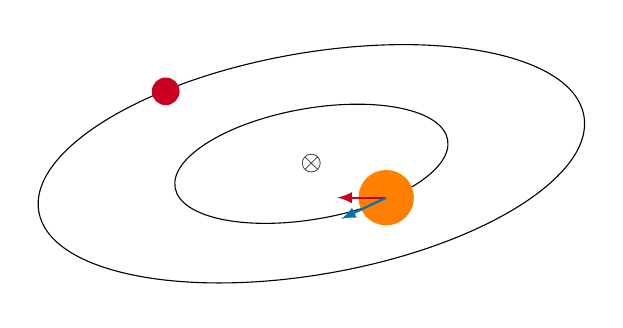
\begin{tikzpicture}[->]
    \draw[rotate=10] (0, 0) ellipse (100pt and 40pt);
    \draw[rotate=10] (0, 0) ellipse (50pt and 20pt);
    \node[draw=none] at (0, 0) (a) {$\otimes$};
    \draw[fill=orange, draw=none] (0.95, -0.43) circle (10pt);
    \draw[color1, line width=\linethickness] (0.95, -0.43) -- (0.33, -0.43);
    \draw[color4, line width=\linethickness] (0.95, -0.43) -- (0.38, -0.70);
    \draw[fill=color1, draw=none] (-1.85, 0.92) circle (5pt);
\end{tikzpicture}
\end{document}
%\documentclass{standalone}
%\usepackage{tikz}
%\usepackage{pgfplots}
%%\usepackage{pgf-spectra}
%
%\def \plotwidth {510.0pt}
%\def \tth{3.16227766017}
%
%\begin{document}
%\begin{tikzpicture}
%\begin{axis}[
%    width=\textwidth, height=240pt,
%%		axis line style={draw=none},
%%		tick style={draw=none},
%	xmin=380, xmax=780,
%	xtick={380, 460, 540, 620, 700, 780},
%	xticklabels={380, 460, 540, 620, 700, 780},
%	yticklabels={},
%]
%%    \put(0, 120pt) {\pgfspectra[lines={400, 500, 550, 700}, absorption, height=20pt, width=\plotwidth/2]}
%%    \put(0, 60pt) {\pgfspectra[lines={395, 495, 545, 695}, absorption, height=20pt, width=\plotwidth/2]}
%%    \put(0, 0pt) {\pgfspectra[lines={390, 490, 540, 690}, absorption, height=20pt, width=\textwidth]}
%\end{axis}
%\end{tikzpicture}
%\end{document}